\documentclass[review,12pt,number]{elsarticle}
% Neural Networks submission format: review = double spacing + line numbers;
% number = numeric citations with elsarticle-num.

\usepackage{amsmath,amssymb}
\usepackage{booktabs}
\usepackage{graphicx}
\usepackage{xcolor}
\usepackage{lineno}
\usepackage{url}
\graphicspath{{figs/}}

\newcommand{\todo}[1]{\textcolor{red}{[TODO: #1]}}
\newcommand{\delp}{DeLP}
\newcommand{\acc}{\mathrm{acc}}
\newcommand{\own}{p_{\mathrm{own}}}

\journal{Neural Networks}

\begin{document}
\linenumbers

\begin{frontmatter}

\title{Segment Specialization in Active-Dendrite Continual Learning:\\
An Audit, an Artifact, and a Causal Repair}

\author[hnucm]{Ranxi Zhou}
\address[hnucm]{Hunan University of Chinese Medicine, 300 Xueshi Avenue,
Hanpu, Yuelu District, Changsha 410208, Hunan, China}
\cortext[cor1]{Corresponding author.}
\ead{zhouranxi@foxmail.com}

\begin{abstract}
Active-dendrite architectures route each input through a competition among
dendritic segments, one of which is trained per task; usage-localized elastic
weight consolidation (\delp{}) protects what has been learned by scaling
per-neutron Fisher anchors with segment usage. Both mechanisms rest on an
implicit assumption that has, to our knowledge, never been measured: that the
segment--task mapping constitutes a \emph{specialization} that protection can
leverage at sub-neuron granularity. We audit this assumption on Permuted-MNIST
and Permuted-Fashion and report three findings. First, a granularity ladder of
anchors (plain, neuron-resolved, segment-resolved with attribution-tracked
reference states) shows that the entire benefit of usage localization is
realized at neuron level: segment-resolved anchors are statistically
indistinguishable from neuron-resolved anchors across every combination of two
datasets, two task counts ($T{=}10,20$), and two elastic weights
($|\Delta\ell|\le 0.24$, all $n{=}10$ paired tests n.s.), and remain so under
FIFO anchor budgets ($|\Delta\ell|\le 0.44$ across eight budget cells).
Second, the audit explains why: task-dominant gating is \emph{absent} ---
among active neurons the probability that a neuron's dominant segment is its
own task's segment starts each phase at chance and is pushed \emph{below}
chance by that phase's own training ($T{=}20$: $0.05 \to 0.01$), and Fisher
mass is diffuse across segments (top-1 share $11$--$18\%$). The audit also
uncovers a measurement artifact relevant to the active-dendrite literature:
under production sampling budgets $56$--$63\%$ of neurons are never activated,
and naive argmax instrumentation over all neurons fabricates a strong
``segment-0 dominance'' ($\approx 60\%$) that vanishes under active-only
filtering. Third, because the missing specialization is load-bearing,
restoring it \emph{causally} improves the retention--plasticity trade-off: a
constant bias on the own-segment dendritic input raises the learning term
in every cell of a $\{$dataset$\}\times\{$depth$\}\times\{$granularity$\}$
grid ($\Delta\ell>0$ in $20/20$ dose cells, significant in $18/20$ at
$n{=}10$ paired), with final accuracy improving in step ($17/20$
simultaneously significant, and every grid cell significant on both terms
at some dose; $\Delta\ell$ up to $+4.6$, $t(9){=}8.1$); forgetting is
reduced at $T{=}10$ ($\Delta\mathrm{BWT}$ up to $+1.7$) and mildly traded
back at $T{=}20$ (significant in $3/8$ cells). Signed-drift
instrumentation shows the network never counteracts the bias at the
parameter level; the own-segment win rate saturates at $0.13$--$0.19$
regardless of dose because any effective dose dominates the raw gate
scale --- partial restoration suffices. Segment--task
specialization in this architecture family is thus not a weak tendency but an
actively violated assumption --- and a repairable one.
\end{abstract}

\begin{keyword}
continual learning \sep elastic weight consolidation \sep active dendrites
\sep dendritic segments \sep catastrophic forgetting \sep interpretability
audit
\end{keyword}

\end{frontmatter}

\linenumbers

% =====================================================================
\section{Introduction}
\label{sec:intro}

Biological neurons integrate thousands of synaptic inputs across morphologically
distinct dendritic compartments, and single-neuron studies have long argued
that these compartments act as quasi-independent computational subunits
\cite{poirazi2003,london2005,poirazi2020}. An influential line of work has
translated this principle into artificial networks: context signals select
one of several dendritic \emph{segments} per neuron, a winner-take-all
competition among segments determines the nonlinear contribution to the
soma, and \emph{only the selected segment receives gradient} on a given task
\cite{iyer2022}. The architectural promise is a division of labor: if task
$k$'s computation flows predominantly through segment $k$, then tasks
naturally occupy disjoint sub-network state, and interference between tasks
has a structural bottleneck.

Continual-learning methods built on dendritic architectures inherit this
promise, often silently. \delp{} (usage-localized elastic weight
consolidation) protects per-neuron parameter blocks with Fisher anchors
scaled by how heavily each neuron was used in past tasks
\cite{zhou2026delp,kirkpatrick2017}. Its protection unit is the neuron; the
segment structure below the neuron is used only to define usage. A natural
proposal --- one we initially expected to succeed --- is to push protection
\emph{down} to the segment level: if tasks really live in different segments,
anchors that track each segment's own reference state should protect more
precisely and drag less on future learning, echoing the granularity
intuition that finer protection localizes interference better.

This paper reports what actually happens when that assumption is tested
rather than assumed. Our contributions are threefold, and each arose from the
failure of the previous one:

\begin{enumerate}
\item \textbf{A granularity audit with a null result at segment level
      (Sec.~\ref{sec:granularity}).} We implement segment-resolved anchors
      with \emph{attribution-tracked reference states} --- each anchor tracks
      where its own segment's parameters drift --- and compare a three-rung
      ladder (plain, neuron-resolved, segment-resolved) across two datasets,
      two depths, and two elastic weights with $n{=}10$ paired seeds. The
      entire benefit of usage localization is realized in the
      plain$\to$neuron step ($\Delta\ell$ between $-2.8$ and $-5.4$,
      $|t(9)|$ up to $22$); the neuron$\to$segment step adds nothing
      ($|\Delta\ell|\le 0.24$, all n.s.), under unbounded stacks and under
      FIFO anchor budgets alike. The null is mechanistically pinned, not
      merely observed: attribution is \emph{self-limiting} (the anchor's own
      penalty pins the weights, so the tracked reference never moves) and
      segment-level parameter ownership lacks a separable carrier.
\item \textbf{A measurement artifact with literature-wide relevance
      (Sec.~\ref{sec:audit}).} Auditing \emph{why} the null occurs, we find
      that under production sampling budgets $56$--$63\%$ of neurons are
      never activated, and that naive dominant-segment instrumentation
      (argmax over segment activations of \emph{all} neurons) attributes
      every dead neuron to segment 0 --- fabricating an apparent
      ``segment-0 dominance'' of $\approx 60\%$ that vanishes under
      active-only filtering. Among active neurons the true picture is
      \emph{anti-specialization}: each phase's own training pushes the
      own-segment win rate from chance to below chance
      ($T{=}20$: $0.05 \to 0.01$), and anchor Fisher mass is diffuse across
      segments (top-1 share $11$--$18\%$). Any study that measures segment
      routing with naive argmax --- including evaluations of segment
      specialization claims --- is at risk of the same artifact.
\item \textbf{A causal repair (Sec.~\ref{sec:causal}).} If missing
      specialization is load-bearing rather than cosmetic, restoring it
      should help. It does: adding a constant bias $b$ to the own-segment
      dendritic input during training, evaluation, and anchor
      construction raises the learning term in every cell of a
      $\{$dataset$\}\times\{$depth$\}\times\{$granularity$\}$ grid ---
      $\Delta\ell$ positive in $20/20$ dose cells, significant in $18/20$
      ($n{=}10$ paired) --- with final accuracy significant simultaneously
      in $17/20$ and in every grid cell at some dose ($\Delta\ell$ up to
      $+4.6$ at $T{=}20$, $t(9){=}8.1$); forgetting is \emph{reduced} at
      $T{=}10$ ($\Delta\mathrm{BWT}$ up to $+1.7$, $t(9)$ up to $10.7$) and
      mildly traded back at $T{=}20$ (significant in $3/8$ cells)
      (Sec.~\ref{sec:causal}). The response is
      saturated and nontrivially mediated: the own-segment win rate
      saturates at $13$--$19\%$ regardless of dose. Signed-drift
      measurement shows this is not adversarial compensation --- the
      network never drifts against the bias --- but a scale effect: the
      raw own gate spans $|u| \le 0.32$, at least three times below any
      tested dose, so the bias forces the same training-time routing at
      every dose, so only a minority of neuron-tasks
      flip to the own-segment pathway --- and that partial restoration
      already yields most of the gain.
\end{enumerate}

Together the three results reframe segment specialization in this
architecture family: not a weak tendency to be exploited, but an
actively violated assumption that can be diagnosed with corrected
instrumentation and partially repaired with a one-parameter intervention.
All experiments are on Permuted-MNIST and Permuted-Fashion at
$T\in\{10,20\}$ with paired-seed statistics; code, per-run records, and
analysis scripts are public (Data Availability).

% =====================================================================
\section{Background and setup}
\label{sec:setup}

\subsection{Active-dendrite network}
\label{sec:adnet}

We use the feed-forward active-dendrite network of Iyer et al.\
\cite{iyer2022} in the protected variant established in our prior work
\cite{zhou2026delp}. A one-hidden-layer network of $N_h$ neurons receives a
one-hot task context $c_t \in \{0,1\}^{T}$; each neuron $j$ carries $T$
dendritic segments, and segment $k$ of neuron $j$ computes
$u_{j,k} = \sigma(w_{(j,k)}^\top x + b_{j,k} + v_{k}^\top c_t)$, where
$v \in \mathbb{R}^{T \times (n_{seg} N_h)}$ are the context-to-dendrite
weights --- \emph{column} $k$ of $v$ gates segment $k$ for every neuron.
The soma nonlinearity applies a $k$-winners-take-all (kWTA) selection over
$h_j = f_j(x)\, \sigma(\max_k u_{j,k})$: the $k$ largest somal pre-activities
pass; the rest are set to zero. Crucially, task $t$'s gradient updates are
masked to the parameters of segment $t$ (``protect\_grads''): the
architecture's design intent is that task $t$ trains segment $t$.

\subsection{\delp{}: usage-localized EWC and the identity decomposition}
\label{sec:delp}

\delp{} \cite{zhou2026delp} protects the feed-forward and output blocks with
per-task anchors, each an elastic penalty
$\frac{\lambda}{2}\sum_p F_p\, (W_p - \theta_p)^2$ whose Fisher term $F$ is
\emph{usage-localized}: per-neuron usage $o_j \in [0,1]$, the frequency with
which neuron $j$ is active under task $t$'s data, scales the anchor rows of
the hidden weights and columns of the output weights, so that rarely-used
neurons are protected lightly and remain available to future tasks. Writing
$\bar a_T$ for final average accuracy, the decomposition
\begin{equation}
\bar a_T \;=\; \ell \;+\; \tfrac{T-1}{T}\,\mathrm{BWT},
\label{eq:identity}
\end{equation}
separates what the \emph{last} task achieves ($\ell$, the learning term)
from what earlier tasks retain (BWT $\le 0$); we report all three, with
paired $t$-statistics over $n{=}10$ seeds sharing permutation streams.

\subsection{Protocol}
\label{sec:protocol}

Benchmarks are Permuted-MNIST and Permuted-Fashion \cite{parisi2019,xiao2017} with
$T\in\{10,20\}$ tasks, one hidden layer of $2000$ neurons, $15$ epochs per
task, Adam (lr $10^{-3}$), Fisher/usage samples of $300$/$500$ examples, and
$\lambda \in \{1000, 5000\}$ calibrated in prior work. Seeds are paired
across arms (identical permutation streams and init); all comparisons are
paired $t$-tests with $n{=}10$, and we mark $|t|>2$ as significant. All
hypotheses in Secs.~\ref{sec:granularity} and \ref{sec:causal} were
preregistered in writing before the corresponding data were collected.

% =====================================================================
\section{Does segment-resolved protection help? A granularity ladder}
\label{sec:granularity}

\subsection{Segment-resolved anchors with attribution-tracked references}
\label{sec:branchdesign}

A segment-resolved anchor must differ from a neuron-resolved one in more
than bookkeeping: since $\sum_k o_{t,j,k} = o_{t,j}$ (segment usages
partition neuron usage), splitting a neuron's single Fisher scalar across
segments while sharing one reference state $\theta$ leaves the penalty
algebraically identical to neuron level. We therefore give each segment
attribution of parameter drift: anchor $a$ (task $t$, neuron $j$) maintains
per-segment reference states $\theta^{(a,k)}$, and after each subsequent
task $t'$ the realized parameter displacement is partitioned across segments
by the usage-driven attribution weights of $t'$'s own anchors; the penalty
charges anchor $a$ only for the drift not explained by interlopers in its
own segment. The design intends that an anchor no longer litigates, on
shared weights, drift caused by tasks that never touched its segment.
Segment-level Fisher mass $m_{t,j,k}$ and dominant-segment histograms are
instrumented per anchor.

\subsection{Result: the ladder is flat above neuron level}

Table~\ref{tab:gran} shows the ladder. The plain$\to$neuron step is large
and universal: at $\lambda{=}1000$, $T{=}10$ MNIST the learning term gains
$+4.66$ ($t(9){=}22.3$); across all six cells of
$\{$dataset$\}\times\{$depth$\}\times\{\lambda\}$, $\Delta\ell$ ranges from
$-2.78$ to $-5.44$ in favor of neuron-level localization with
$|t(9)| \in [10.4, 22.3]$. The neuron$\to$segment step is empty: the
largest deviation across all twelve pairings is $|\Delta\ell| = 0.24$,
never significant (largest $|t| = 1.3$); BWT differences are within
$0.4$ points.

\begin{table}[t]
\centering\footnotesize\setlength{\tabcolsep}{4.5pt}
\caption{Granularity ladder (unbounded anchor stacks, $n{=}10$ paired
seeds). $\ell$/avg/BWT are absolute means; the right block is the paired
difference vs.\ the neuron-resolved arm. All plain$-$neuron differences are
significant at $|t|>10$; no branch$-$neuron difference is significant
(largest $|t| = 1.3$).}
\label{tab:gran}
\begin{tabular}{llrrrr rr}
\toprule
 & & \multicolumn{3}{c}{absolute means} & \multicolumn{3}{c}{paired vs.\ neuron} \\
\cmidrule(lr){3-5}\cmidrule(lr){6-8}
cell & arm & $\ell$ & avg & BWT & $\Delta\ell$ & $\Delta$avg & $\Delta$BWT \\
\midrule
\multicolumn{8}{l}{\emph{Permuted-MNIST, $\lambda{=}1000$}}\\
$T{=}10$ & plain  & 69.63 & 61.25 & $-9.31$ & $-4.66^{*}$ & $-2.61^{*}$ & $+2.26^{*}$ \\
$T{=}10$ & neuron & 74.28 & 63.86 & $-11.58$ & --- & --- & --- \\
$T{=}10$ & branch & 74.21 & 64.13 & $-11.20$ & $-0.08$ & $+0.27$ & $+0.38$ \\
$T{=}20$ & plain  & 46.35 & 37.30 & $-9.53$ & $-5.44^{*}$ & $-1.35^{*}$ & $+4.31^{*}$ \\
$T{=}20$ & neuron & 51.79 & 38.64 & $-13.84$ & --- & --- & --- \\
$T{=}20$ & branch & 51.98 & 39.03 & $-13.63$ & $+0.19$ & $+0.39$ & $+0.21$ \\
\midrule
\multicolumn{8}{l}{\emph{Permuted-MNIST, $\lambda{=}5000$}}\\
$T{=}10$ & plain  & 54.41 & 51.69 & $-3.03$ & $-4.78^{*}$ & $-2.80^{*}$ & $+2.19^{*}$ \\
$T{=}10$ & neuron & 59.19 & 54.49 & $-5.22$ & --- & --- & --- \\
$T{=}10$ & branch & 59.21 & 54.71 & $-5.01$ & $+0.03$ & $+0.22$ & $+0.21$ \\
$T{=}20$ & plain  & 33.97 & 31.68 & $-2.40$ & $-3.72^{*}$ & $-1.74^{*}$ & $+2.08^{*}$ \\
$T{=}20$ & neuron & 37.68 & 33.42 & $-4.49$ & --- & --- & --- \\
$T{=}20$ & branch & 37.59 & 33.39 & $-4.42$ & $-0.09$ & $-0.03$ & $+0.07$ \\
\midrule
\multicolumn{8}{l}{\emph{Permuted-Fashion, $\lambda{=}5000$}}\\
$T{=}10$ & plain  & 38.53 & 33.47 & $-5.62$ & $-3.76^{*}$ & $-1.65^{*}$ & $+2.35^{*}$ \\
$T{=}10$ & neuron & 42.29 & 35.12 & $-7.96$ & --- & --- & --- \\
$T{=}10$ & branch & 42.05 & 35.27 & $-7.53$ & $-0.24$ & $+0.15$ & $+0.43$ \\
$T{=}20$ & plain  & 26.56 & 22.75 & $-4.01$ & $-2.78^{*}$ & $-1.22^{*}$ & $+1.65^{*}$ \\
$T{=}20$ & neuron & 29.35 & 23.97 & $-5.66$ & --- & --- & --- \\
$T{=}20$ & branch & 29.35 & 24.14 & $-5.49$ & $+0.01$ & $+0.17$ & $+0.17$ \\
\bottomrule
\end{tabular}
\end{table}

Single-anchor references (Table~\ref{tab:refs}) frame the arms; their
$\lambda$ values are the calibration carried over from our companion
pipeline, not re-tuned per benchmark. Plain EWC buys $\ell$ at
$3$--$5\times$ the forgetting; SI ($\lambda{=}100$) is over-stable (its
$\ell{=}13$ at $T{=}10$ shows it barely learns later tasks at all); MAS
($\lambda{=}1$) maximizes the learning term ($\ell \ge 87$, the highest
of all arms) yet posts catastrophic BWT ($-32.6$ at $T{=}20$) --- the
regime-dependence of warrant documented in our companion work extends
from Split-CIFAR-100 to the MLP setting. One comparison the table makes
possible is worth stating explicitly: at $T{=}10$, the repaired
\mbox{DeLP} arm ($b{=}10$; avg $68.7$, BWT $-9.9$) dominates MAS (avg
$66.6$, BWT $-21.2$) on both summary terms --- MAS buys its higher
learning term with exactly the forgetting that the repair removes.

\begin{table}[t]
\centering\small
\caption{Single-anchor references (Permuted-MNIST, $n{=}10$).}
\label{tab:refs}
\begin{tabular}{llrrr}
\toprule
 & method ($\lambda$) & $\ell$ & avg & BWT \\
\midrule
$T{=}10$ & SI ($100$) & 13.23 & 39.26 & $-0.83$ \\
$T{=}10$ & MAS ($1$)   & 87.00 & 66.61 & $-21.21$ \\
$T{=}20$ & SI ($100$) & 11.19 & 25.14 & $-0.69$ \\
$T{=}20$ & MAS ($1$)   & 87.91 & 55.75 & $-32.56$ \\
\bottomrule
\end{tabular}
\end{table}

\subsection{The flatness survives anchor budgets}
\label{sec:budget}

Because segment-resolved anchors might pay off only when the anchor
\emph{stack} is bounded --- fewer anchors plausibly sharpen the value of
each --- we crossed granularity with FIFO budgets $M \in \{2, 5\}$ at
$\lambda{=}1000$ (preregistered: alive iff $\ge 4/6$ cells significant
positive and none significantly worse on BWT). The result is the same null,
tighter: across all eight $\{$dataset$\}\times\{M\}\times\{T\}$ cells the
branch$-$neuron $\Delta\ell$ lies within $\pm 0.44$ with no cell significant
positive (one cell, Fashion $M{=}2$, $T{=}10$, is significantly
\emph{negative} at $-0.33$, $t(9){=}-2.3$; Table~\ref{tab:budget}).
Budgets shift both granularities identically, consistent with the shared
mechanism analysis below.

\begin{table}[t]
\centering\small
\caption{Granularity under FIFO anchor budgets ($\lambda{=}1000$, $n{=}10$
paired). No branch$-$neuron difference is significant positive in any of
the eight cells.}
\label{tab:budget}
\begin{tabular}{llrrrr}
\toprule
cell & $M$ & neuron $\ell$ & branch $\ell$ & $\Delta\ell$ (t) & $\Delta$BWT (t) \\
\midrule
MNIST $T{=}10$  & 2 & 83.06 & 83.01 & $-0.05\;(-1.0)$ & $+0.22\;(+0.9)$ \\
MNIST $T{=}10$  & 5 & 77.09 & 77.02 & $-0.07\;(-0.5)$ & $+0.16\;(+0.7)$ \\
MNIST $T{=}20$  & 2 & 80.23 & 80.32 & $+0.09\;(+1.0)$ & $+0.39\;(+0.9)$ \\
MNIST $T{=}20$  & 5 & 68.30 & 68.19 & $-0.11\;(-0.8)$ & $+0.29\;(+1.0)$ \\
Fashion $T{=}10$ & 2 & 66.66 & 66.33 & $-0.33\;(-2.3)^{*}$ & $-0.40\;(-1.0)$ \\
Fashion $T{=}10$ & 5 & 58.90 & 58.74 & $-0.16\;(-0.9)$ & $+0.43\;(+1.2)$ \\
Fashion $T{=}20$ & 2 & 62.61 & 62.72 & $+0.10\;(+0.4)$ & $-0.18\;(-0.4)$ \\
Fashion $T{=}20$ & 5 & 49.79 & 50.23 & $+0.44\;(+1.5)$ & $-0.33\;(-0.7)$ \\
\bottomrule
\end{tabular}
\end{table}

% =====================================================================
\section{Why the ladder is flat: auditing segment--task specialization}
\label{sec:audit}

The null in Sec.~\ref{sec:granularity} would be easy to misread as ``the
segment machinery is redundant.'' The audit says something stronger: the
specialization that segment-resolved protection would need does not exist,
and part of the evidence that appeared to show it was an artifact.

\subsection{A measurement artifact: dead neurons fabricate dominance}
\label{sec:artifact}

Our first-pass instrumentation recorded, for every neuron, the argmax over
its segment activations under each task's data. It showed segment 0
``dominating'' $58$--$63\%$ of neurons --- a striking positional bias that
initially looked like the failure of task-specific routing. The correction:
under the production sampling budget ($500$ examples), $56$--$63\%$ of
neurons are \emph{never activated}; for a dead neuron all segment
activations are exactly zero, argmax breaks ties toward index $0$, and the
neuron is silently booked to segment 0 (Fig.~\ref{fig:artifact}).
Filtering to active neurons collapses the apparent bias to chance
($\approx 0.10 = 1/T$ at $T{=}10$; untrained networks show no positional
preference either, $0.096$--$0.111$ over three seeds). The death itself is
real and grows with the sequence: the inactive fraction jumps from $0.02$
to $0.35$ within the first phase of training and stabilizes near $0.6$
(Fig.~\ref{fig:deadfrac}) --- under kWTA, neurons pushed out of the
winner set early are never re-selected by any later task. We flag this as
a methodological warning for the active-dendrite literature: dominance
statistics computed over all neurons conflate routing with mortality, and
at production sampling budgets the conflation is an order of magnitude
larger than the signal.

\begin{figure}[t]
\centering
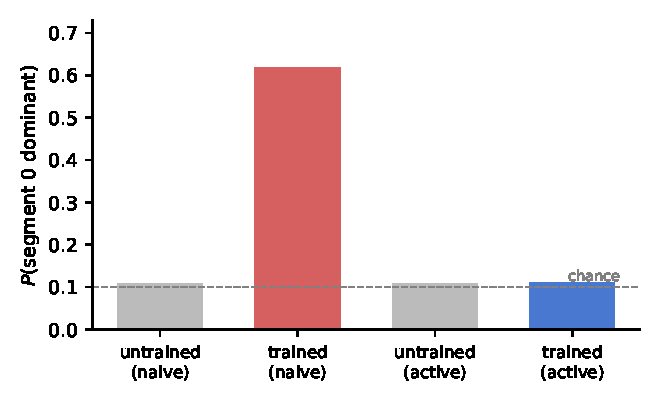
\includegraphics[width=.55\linewidth]{fig_artifact.pdf}
\caption{The dead-neuron artifact. Naive argmax over \emph{all} neurons
reports segment-0 dominance of $\approx 60\%$ after training; the same
statistic over active neurons only, and both statistics on untrained
networks, sit at chance ($1/T$).}
\label{fig:artifact}
\end{figure}

\begin{figure}[t]
\centering
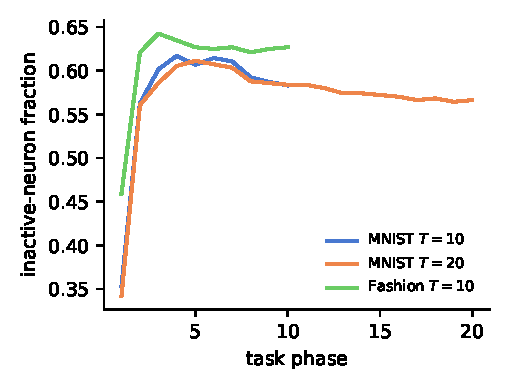
\includegraphics[width=.5\linewidth]{fig_deadfrac.pdf}
\caption{Inactive-neuron fraction across the task sequence (end-of-phase
means). Neurons lost in early phases are never recovered; the active
substrate available to routing is roughly halved by phase 2 and
stabilizes near $40\%$.}
\label{fig:deadfrac}
\end{figure}

\subsection{Anti-specialization among active neurons}
\label{sec:anti}

With the artifact controlled, the true routing picture is the opposite of
specialization. Define $\own$ as the probability that a neuron's dominant
segment is the currently measured task's own segment, over active neurons.
At the \emph{start} of each phase, $\own$ sits at chance ($1/T$): nothing
in the context-gated routing maps tasks to segments. Training within the
phase then pushes it \emph{below} chance --- by the end of phase $p$, $\own$
drops to $0.058$--$0.085$ at $T{=}10$ (chance $0.10$) and, late in a
$T{=}20$ sequence, to $0.005$--$0.02$ against a chance of $0.05$, i.e.\ five
to ten times \emph{below} random assignment (Fig.~\ref{fig:evolution}).
The own-segment gating block does train --- it moves by $6$--$16\%$ of its
norm per phase --- yet this movement fails to convert into dominance: win
rates still end each phase below chance. Segment--task alignment is not
merely absent; its absence persists through active training of the very
parameters that would encode it.

\begin{figure}[t]
\centering
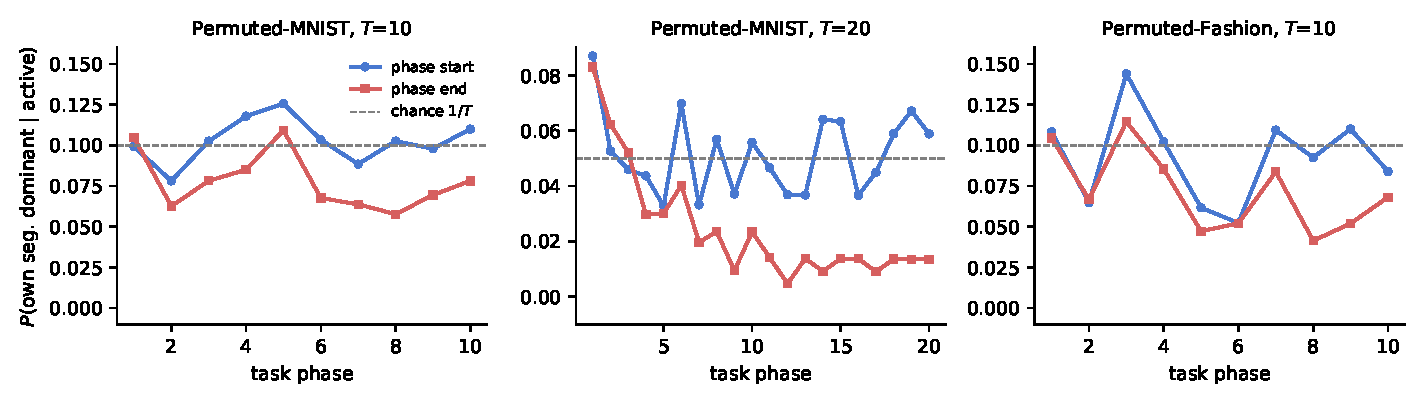
\includegraphics[width=\linewidth]{fig_evolution.pdf}
\caption{Anti-specialization over training. Within each phase, the
own-segment win rate over active neurons starts at chance (dashed) and
ends below it; the deficit deepens with sequence position (rightmost
points of each curve), most severely at $T{=}20$.}
\label{fig:evolution}
\end{figure}

\subsection{Fisher mass is diffuse across segments}

Segment-resolved anchors also lack a substrate to hold onto: for trained
anchors, the fraction of a neuron's Fisher mass attributable to its top
segment is only $11$--$18\%$ (mean over anchor--neuron pairs). Even a
perfectly attributed segment-level penalty would spread nearly all of its
protection across segments the anchor task never drove. This measurement
closes the mechanistic account of the Sec.~\ref{sec:granularity} null from
two sides: attribution is self-limiting (an anchor's own penalty pins the
shared weights it measures, so its tracked references barely move), and
the per-segment mass that attribution would partition is diffuse to begin
with.

% =====================================================================
\section{Causal probe: restoring own-segment advantage}
\label{sec:causal}

\subsection{A one-parameter intervention}

If the missing specialization is load-bearing, causally restoring it should
improve the trade-off in Eq.~\eqref{eq:identity}. We add a constant bias $b$
to the own-segment dendritic input: $u_{j,t} \mathrel{+}= b$ whenever the
context selects task $t$. The bias is active in training, evaluation, and
anchor construction (the Fisher measurement that drives usage-localized
protection); the dominant-segment win-rate instrument deliberately reads
the raw, bias-free gates, so that every routing statistic in this paper
describes what the network itself encodes rather than what the bias
forces (Sec.~\ref{sec:compensation}). The intervention is deliberately
dumb --- no learned parameters, no schedule, no per-neuron structure ---
so that any effect is attributable to the routing prior alone. Doses
$b \in \{0, 1, 3, 10\}$; all comparisons paired against $b{=}0$ on
identical seeds.

\subsection{Result: the learning term and accuracy improve everywhere}

Tables~\ref{tab:dose10} and \ref{tab:dose20} give the dose--response;
Fig.~\ref{fig:dose} plots it. Across the $20$ dose cells of the
$\{$dataset$\}\times\{$depth$\}\times\{$granularity$\}$ grid with
$b \ge 1$, $\Delta\ell$ is positive in every cell and significant in
$18/20$; $\ell$ and final accuracy are simultaneously significant in
$17/20$, and every grid cell has at least one dose significant on both
terms. The effect grows with depth: at $T{=}20$ MNIST, $b{=}10$ lifts
$\ell$ by $+4.56$ ($t(9){=}8.1$) and final accuracy by $+3.81$
($t(9){=}10.6$) over the already usage-localized baseline. Forgetting
improves broadly at $T{=}10$ ($\Delta\mathrm{BWT}$ up to $+1.65$;
significantly positive in $8/12$ cells, and in all six MNIST cells), and
partially trades back at $T{=}20$, where $3/8$ cells show a significant
mild BWT cost ($-0.66$ to $-0.95$) and the remaining five are
statistically indistinguishable from baseline.

Two robustness notes. First, the $20/20$ sign uniformity of $\Delta\ell$
is itself the strongest guard against multiplicity: a sign test gives
$p = 2^{-20}$, orders of magnitude below any family-wise correction over
the grid. Second, the intervention also reduces neuron mortality ---
measured on the raw, bias-free network, the mean dead fraction drops by
$3.9$pp (MNIST) and $2.3$pp (Fashion) at $T{=}10$ --- and per-run
$\Delta\ell$ correlates with the mortality reduction ($r{=}-0.49$ and
$-0.68$). We read this as one causal chain rather than a confound:
raising the own-segment gate raises $\mathrm{sigmoid}(u)$ during
training, which increases kWTA survival, so forcing the routing prior is
also what keeps neurons alive; the routing and capacity channels are two
faces of a single intervention, not competing explanations.

\begin{table}[t]
\centering\small
\caption{Causal probe, $T{=}10$, $\lambda{=}1000$: paired differences vs.\
$b{=}0$ ($n{=}10$; $^{*}$: $|t|>2$). $\own$ is the own-segment win rate
over active neurons, averaged over phases.}
\label{tab:dose10}
\begin{tabular}{llrrrr r}
\toprule
dataset & arm ($b$) & $\Delta\ell$ & $\Delta$avg & $\Delta$BWT & $\own$ \\
\midrule
MNIST & neuron ($1$)  & $+1.99^{*}$ & $+3.40^{*}$ & $+1.56^{*}$ & 0.19 \\
MNIST & neuron ($3$)  & $+2.68^{*}$ & $+4.08^{*}$ & $+1.56^{*}$ & 0.17 \\
MNIST & neuron ($10$) & $+3.32^{*}$ & $+4.80^{*}$ & $+1.65^{*}$ & 0.16 \\
MNIST & branch ($10$) & $+3.16^{*}$ & $+4.17^{*}$ & $+1.13^{*}$ & 0.16 \\
Fashion & neuron ($1$)  & $+0.87$ & $+1.03$ & $+0.18$ & 0.15 \\
Fashion & neuron ($3$)  & $+1.23^{*}$ & $+2.56^{*}$ & $+1.48^{*}$ & 0.14 \\
Fashion & neuron ($10$) & $+1.39^{*}$ & $+0.69$ & $-0.77$ & 0.13 \\
Fashion & branch ($3$)  & $+0.81$ & $+1.79^{*}$ & $+1.09^{*}$ & 0.14 \\
\bottomrule
\end{tabular}
\end{table}

\begin{table}[t]
\centering\small
\caption{Causal probe, $T{=}20$: paired differences vs.\ $b{=}0$
($n{=}10$; $^{*}$: $|t|>2$).}
\label{tab:dose20}
\begin{tabular}{llrrrr r}
\toprule
dataset & arm ($b$) & $\Delta\ell$ & $\Delta$avg & $\Delta$BWT & $\own$ \\
\midrule
MNIST & neuron ($3$)  & $+3.72^{*}$ & $+3.25^{*}$ & $-0.49$ & 0.14 \\
MNIST & neuron ($10$) & $+4.56^{*}$ & $+3.81^{*}$ & $-0.79^{*}$ & 0.13 \\
MNIST & branch ($3$)  & $+3.66^{*}$ & $+3.03^{*}$ & $-0.66^{*}$ & 0.14 \\
MNIST & branch ($10$) & $+4.13^{*}$ & $+3.48^{*}$ & $-0.68$ & 0.13 \\
Fashion & neuron ($3$)  & $+2.19^{*}$ & $+2.09^{*}$ & $-0.11$ & 0.14 \\
Fashion & neuron ($10$) & $+1.94^{*}$ & $+1.03^{*}$ & $-0.95^{*}$ & 0.13 \\
Fashion & branch ($3$)  & $+1.44^{*}$ & $+1.98^{*}$ & $+0.57$ & 0.13 \\
Fashion & branch ($10$) & $+2.18^{*}$ & $+1.96^{*}$ & $-0.24$ & 0.13 \\
\bottomrule
\end{tabular}
\end{table}

\begin{figure}[t]
\centering
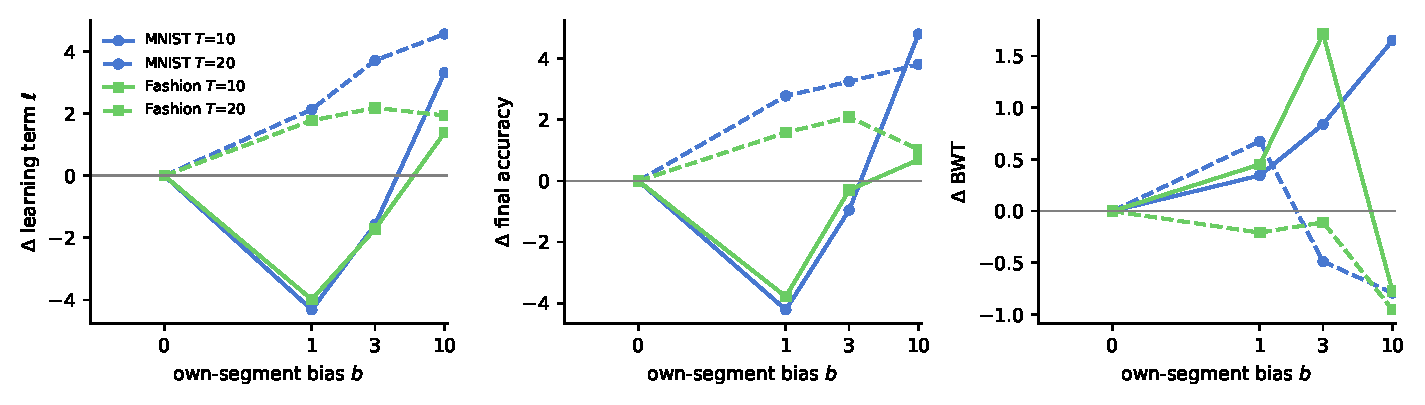
\includegraphics[width=\linewidth]{fig_dose.pdf}
\caption{Dose--response of the own-segment bias (neuron-resolved arm,
paired means vs.\ $b{=}0$). The learning term (left) and final accuracy
(middle) improve at every dose, dataset, and depth; BWT (right) improves
at $T{=}10$ and is mildly negative at $T{=}20$ on MNIST. Note the
saturating shape: $b{=}3$ alone already captures most of the $b{=}10$
effect ($81$--$113\%$ across datasets and depths).}
\label{fig:dose}
\end{figure}

\subsection{The intervention is absorbed, not opposed}
\label{sec:compensation}

The mediation of the effect is as informative as its size. The bias does
\emph{not} flip measured routing: the own-segment win rate rises only from
$\approx 0.08$ to a saturated $0.13$--$0.19$, and is nearly insensitive
to a tenfold dose increase ($b{=}1$: $0.19$; $b{=}3$: $0.17$; $b{=}10$:
$0.16$). The dose-invariance has a scale explanation rather than an
adversarial one. The raw own-segment gate that the win-rate instrument
reads stays within $|u| \le 0.32$ across all seeds and phases (seed
means within $\pm 0.16$; Sec.~\ref{sec:sigdrift}); every tested dose is
at least three times this range, so the bias, not the raw gate,
determines the own segment's training-time advantage. The resulting
parameter-level trace is dose-invariant, and hence so is the measured
win rate. Signed-drift measurement
(Sec.~\ref{sec:sigdrift}) confirms that the network never counteracts
the bias at the parameter level: the own gating column drifts
\emph{positive}, not negative, under the imposed bias. Two conclusions
follow. First, the improvement is not an artifact of forcing hard
routing --- the measured routing solution survives essentially intact.
Second, only a minority of neurons needs to respect the segment--task
prior for the retention--plasticity balance to shift significantly:
specialization operates as a bottleneck resource, and partial
restoration is sufficient.

\subsection{Signed drift: no pushback at the parameter level}
\label{sec:sigdrift}

To test whether the saturation above reflects the learner undoing the
bias, we re-ran the $T{=}10$ MNIST probe with per-phase signed
instrumentation of the context-$t$ gating column (own-segment entries),
under $b{=}0$ and $b{=}10$ ($n{=}3$ seeds). Adversarial compensation
predicts a systematic \emph{negative} displacement of the own gating
column in the bias-imposed runs. The measurement shows the opposite.
Under $b{=}10$ the own-segment entries drift \emph{positive} in all ten
phases (one-sample $t$ over seeds: $223$, $37$, $17$, $17$, $8$, $11$,
$9$, $5.1$, $4.4$, $4.5$; per-phase mean displacement decaying from
$+0.027$ to $+0.004$), versus $\le +0.004$ under $b{=}0$, significant
only in the first two phases. The raw own gate stays within
$|u| \le 0.32$ across all seeds and phases (seed means within
$\pm 0.16$) --- thirty times below the imposed $b{=}10$ and three times
below even $b{=}1$ --- so the offset remains fully in effect throughout
training. The network absorbs the intervention instead of opposing it:
task training reinforces the forced own-segment routing slightly, and
the ceiling of the measured win rate is a property of the raw-gate
scale, not of active compensation. A complementary probe asks whether
the network would learn the bias on its own; it acquires only a small
positive own-segment bias at the raw-gate scale, an order of magnitude
below the smallest effective dose (Sec.~\ref{sec:limitations}).

\subsection{Why forgetting trades back at depth}
\label{sec:depthbwt}

At $T{=}10$ the bias reduces forgetting; at $T{=}20$ MNIST it mildly
increases it. The probe's measurement explains the sign flip. With the
bias active, a fixed minority of neurons routes through the own segment in
\emph{every} phase; over a longer sequence, later phases increasingly
share this minority substrate, so late-task updates overlap earlier
anchors on the same (now doubly used) neurons --- $\ell$ rises because
more neurons are available early, but the shared minority pays for it at
depth. The saturation of $\own$ (Sec.~\ref{sec:compensation}) caps how
much substrate the repair can recruit; at $T{=}20$ the cap binds.

% =====================================================================
\section{Related work}
\label{sec:related}

\paragraph{Active-dendrite networks.} Single-neuron compartmental models
\cite{poirazi2003,london2005,poirazi2020,ujfalussy2018} motivate
multi-segment artificial neurons; Iyer et al.\ \cite{iyer2022} operationalize
context-gated segment competition for lifelong classification and report
reduced interference, and the GWC route-suppression variant
\cite{boyle2025,baek2024} and neuromorphic implementations
\cite{boahen2022} extend the family. These works validate the architecture;
to our knowledge none measures whether the intended segment--task
specialization actually obtains in the trained model, which is the object
of our audit --- nor, consequently, the dead-neuron artifact that
naive dominance statistics incur under production sampling budgets.

\paragraph{Elastic weight consolidation and its localizations.} EWC
\cite{kirkpatrick2017} protects parameters with a single global anchor;
SI \cite{zenke2017}, MAS \cite{aljundi2018}, and online variants
\cite{chaudhry2018} refine the importance estimate; masking approaches
\cite{mallya2018,serra2018,masse2018} hard-allocate capacity. \delp{}
\cite{zhou2026delp} localizes EWC per neuron via usage, and our companion
work diagnoses the anchor-accumulation problem and bounds the anchor stack
\cite{zhou2026delp}. The present study is orthogonal: it asks whether
protection granularity should descend \emph{below} the neuron and answers
negatively, then explains the negative via a routing audit and repairs the
routing instead.

\paragraph{Negative results and measurement validity.} Benchmark pitfalls
\cite{musgrave2020,lucic2018,melis2018,agarwal2021,lipton2019} established
that evaluation practice can manufacture effects; the dead-neuron artifact
here is an instance inside the model rather than the benchmark: the
instrumentation, not the metric, fabricates the signal.

% =====================================================================
\section{Limitations}
\label{sec:limitations}

\begin{enumerate}
\item \textbf{Scale.} All results are on one-hidden-layer MLPs with
      permuted benchmarks and $T \le 20$. The artifact and
      anti-specialization findings concern the interaction of kWTA
      mortality with argmax instrumentation and should be re-checked
      wherever segments exist (e.g.\ convolutional or transformer backbones
      with routing modules); the causal repair's transfer is untested
      beyond this family.
\item \textbf{The repair is a prior, not a mechanism.} The constant bias
      encodes the correct assumption (own segment first) that the network
      fails to learn at effective strength. We measured this directly:
      given a trainable per-(task, segment) bias table initialized at
      zero, the network acquires only a small positive own-segment bias
      ($+0.113 \pm 0.031$ MNIST, $+0.083 \pm 0.025$ Fashion; $n{=}7$
      runs each, $t(6) \ge 8.7$) --- the raw-gate scale, an order of
      magnitude below the smallest effective dose --- and its accuracy
      matches the unbiased baseline. A learned or annealed intervention
      might avoid the depth trade-off (Sec.~\ref{sec:depthbwt}); we
      deliberately did not tune one, to keep the causal claim clean.
\item \textbf{Depth-dependent forgetting trade-off.} At $T{=}20$ the BWT
      cost of the bias is small but real: $3/8$ cells significantly
      negative ($-0.66$ to $-0.95$), the rest indistinguishable from
      baseline. We
      report it rather than select it away; the identity
      Eq.~\eqref{eq:identity} makes explicit that accuracy gains can
      coexist with mildly worse retention.
\item \textbf{Granularity null is architecture-bound.} The
      plain$\to$neuron step's dominance may weaken in architectures where
      segment parameters are genuinely disjoint (no shared feed-forward
      weights); our null is about this family's shared-substrate design.
\end{enumerate}

% =====================================================================
\section{Conclusion}
\label{sec:conclusion}

We asked whether the segment structure of active-dendrite networks offers
protection granularity below the neuron, and found that the question
dissolves one level up: the entire benefit of usage-localized protection is
realized at neuron level because the segment--task specialization the finer
granularity would need is absent --- measured, at chance before each phase
and pushed below chance by each phase's own training, with Fisher mass too
diffuse to partition meaningfully. On the way we isolated a dead-neuron
artifact that fabricates dominance statistics for any naive instrument in
this family, and showed that a one-parameter causal repair of the routing
prior raises the learning term in every tested cell (significant in
$18/20$ dose cells), with the network itself revealing --- through a
dose-invariant saturated minority flip --- that specialization is a scarce
resource worth a little, but only a little. Auditing the assumption before
building on it took one paper's worth of null results; we hope the
corrected instrumentation and the repair make the next one shorter.

% =====================================================================
\section*{Data availability}
All code, per-run records (JSON), and analysis scripts are available at
\url{https://github.com/zhouranxi/delp-anchor-budget} (experiments
\texttt{s1\_*}, \texttt{gevo\_*}, \texttt{c2*}; figures via
\texttt{paper\_s1/make\_figs.py}).

\section*{Declaration of competing interest}
The author declares no competing interests.

\bibliographystyle{elsarticle-num}
\bibliography{refs}

\end{document}
